% RUG LaTeX Template %
% Author: Konstantine Gkaras
% E-mail: kgaras041@gmail.com // k.gkaras@student.rug.nl
% Created: Sat 19 Oct 2024 @ 00:30:12 +0200
% Modified: Sat 29 Mar 2025 @ 13:05:40 +0100

\documentclass{article}

%%%%%%%%%%%%%%%%%%%%%%%%%%%%%%%%%%%%%%%%%%%%%%%%%%%%%%%%%%%%%%%%%%%%
%%-----------------------PAGE SETTINGS----------------------------%%
%%%%%%%%%%%%%%%%%%%%%%%%%%%%%%%%%%%%%%%%%%%%%%%%%%%%%%%%%%%%%%%%%%%%
\usepackage[utf8]{inputenc}
\usepackage[margin=0.01cm]{geometry}

%%%%%%%%%%%%%%%%%%%%%%%%%%%%%%%%%%%%%%%%%%%%%%%%%%%%%%%%%%%%%%%%%%%%
%%--------------------------PREAMBLE------------------------------%%
%%%%%%%%%%%%%%%%%%%%%%%%%%%%%%%%%%%%%%%%%%%%%%%%%%%%%%%%%%%%%%%%%%%%
\usepackage{pdfpages}                           % Insert PDF into file without breaking margins and print output.
\usepackage{anyfontsize}                        % Use any font size.
\usepackage{setspace}                           % Customize paragraph spacing.
\usepackage{mathtools}                          % Math typing.
\usepackage{cancel}                             % Strikethrough text.
\usepackage{float}                              % Force figure on position.
\usepackage{hyperref}				            % Links.
\usepackage{amsmath}                            % Math typing.
\usepackage{inputenc}                           % Special characters.
\usepackage{amsfonts}                           % Fontpack.
\usepackage{graphicx}                           % Graphics.
\usepackage{enumitem}                           % Special numerisation on lists.
\usepackage{amsthm}                             % Math.
\usepackage{xcolor}                             % Colors.
\usepackage{lipsum}                             % Dummy text.
\usepackage{url}								% Url's.
\usepackage{lmodern}							% Latin Modern for Computer Fonts.
\usepackage{textcomp}							% Special symbols like degrees or euro.
\usepackage{listings}							% Input code directly from file or path.
\usepackage{pdfpages}							% Include pdf documents in the output file.
\usepackage{amssymb}							% Math.
\usepackage{tikz}								% Drawing plots.
\usetikzlibrary{shapes.geometric, arrows}		% Select tikz library.

%%%%%%%%%%%%%%%%%%%%%%%%%%%%%%%%%%%%%%%%%%%%%%%%%%%%%%%%%%%%%%%%%%%%
%%-----------------------CUSTOM COMMANDS--------------------------%%
%%%%%%%%%%%%%%%%%%%%%%%%%%%%%%%%%%%%%%%%%%%%%%%%%%%%%%%%%%%%%%%%%%%%
\newcommand{\textBF}[1]{%
    \pdfliteral direct {2 Tr 1 w}               %the second factor is the boldness
     #1%
    \pdfliteral direct {0 Tr 0 w}               %
}

\newcommand{\textDF}[1]{%
    \pdfliteral direct {2 Tr 0.2 w}             %the second factor is the boldness
     #1%
    \pdfliteral direct {0 Tr 0 w}               %
}

\definecolor{codegreen}{rgb}{0,0.6,0}
\definecolor{codegray}{rgb}{0.5,0.5,0.5}
\definecolor{codepurple}{rgb}{0.58,0,0.82}
\definecolor{backcolour}{rgb}{0.95,0.95,0.92}

\lstdefinestyle{mystyle}{
    backgroundcolor=\color{backcolour},   
    commentstyle=\color{codegreen},
    keywordstyle=\color{magenta},
    numberstyle=\tiny\color{codegray},
    stringstyle=\color{codepurple},
    basicstyle=\ttfamily\footnotesize,
    breakatwhitespace=false,         
    breaklines=true,                 
    captionpos=b,                    
    keepspaces=true,                 
    numbers=left,                    
    numbersep=5pt,                  
    showspaces=false,                
    showstringspaces=false,
    showtabs=false,                  
    tabsize=2
}

\lstset{style=mystyle}

% Define the abs() function
\newcommand{\abs}[1]{\left\lvert #1 \right\rvert}

% Define the norm() function
\newcommand{\norm}[1]{\left\lVert #1 \right\rVert}

% Define the inner product using angle brackets
\newcommand{\inner}[2]{\left\lange #1, #2 \right\rangle}

% Define the argmin operator
\DeclareMathOperator*{\argmin}{argmin}

% Define the dist operator
\DeclareMathOperator*{\dist}{dist}

% Define the resolvent operator
\DeclareMathOperator{\res}{Res}

% Define the proximal operator
\DeclareMathOperator*{\prox}{prox}

% Redefine the proof environment to be completely silent
\renewenvironment{proof}%
{\noindent}%
{\hfill$\square$\par}

% Start section counter from 0
%\setcounter{section}{-1}

%%%%%%%%%%%%%%%%%%%%%%%%%%%%%%%%%%%%%%%%%%%%%%%%%%%%%%%%%%%%%%%%%%%%
%%-----------------------DOCUMENT BEGIN---------------------------%%
%%%%%%%%%%%%%%%%%%%%%%%%%%%%%%%%%%%%%%%%%%%%%%%%%%%%%%%%%%%%%%%%%%%%
\begin{document}

\begin{titlepage}
\thispagestyle{empty}
\title{
\includegraphics[width=19cm]{Extras/Mathlogo.PNG} \\
\vspace{3cm}
\begingroup
\setstretch{4}\fontsize{20}{10}\selectfont\fontdimen2\font=0.8ex
% Project Title  %
% If you want the title centered, leave the command as it is, 
% otherwise delete the \center{} command.
\parbox{15cm}{\center{\textBF{Heuristic Approaches to Real-World Optimization: A Case Study on the Travelling Salesman Problem}}}
\endgroup}
\date{}
\maketitle
\vspace{-1.5cm}
\hspace{4cm}\parbox[b][15cm][b]{10cm}{\textDF{\large\setstretch{1.5}
Mathematics and its Environment \\
\date{\today}\\
Student: Konstantinos Gkaras\\ %NAME
Student Number: S5941814
}}
\end{titlepage}
\newpage
% Define new page geometry because the default was changed for title page.
\newgeometry{top=1in,bottom=1in,right=1in,left=1in}

% Table of contents
\tableofcontents

% Input document sub-files, following the divide and conquer strategy.
% Abstract of the Final Essay for Math & Environment %
% Author: Konstantinos Garas
% E-mail: kgaras041@gmail.com // k.gkaras@student.rug.nl
% Created: Fri 28 Mar 2025 @ 13:49:42 +0100
% Modified: Fri 28 Mar 2025 @ 14:07:26 +0100

\begin{abstract}
	This report studies the computational comparisons of the most famous numerical heuristic schemes (NN, GA, SA, ACO) that solve the Travelling Salesman Problem (TSP). First, this discrete optimization problem is introduced, alongside some required simplifications. Then, the basic idea of each heuristic scheme is described, with the goal to establish a difficulty baseline between these algorithms. Lastly, these methods are put to the test for 30 randomly generated case studies of graphs with 229 cities, which is equivalent in essence as trying to solve the real-world problem for the Netherlands. The results favour the Ant Colony Optimization (ACO) heuristic scheme, and showcase that complexity of ideas doesn't necessarily translate to better results.
\end{abstract}

Keywords---Travelling Salesman Problem, heuristic algorithms, Nearest Neighbor (NN), Genetic Algorithm (GA), Simulated Annealing (SA), Ant Colony Optimization (ACO).
			% abstract
% Introduction of the Final Essay for Math & Environment %
% Author: Konstantinos Garas
% E-mail: kgaras041@gmail.com // k.gkaras@student.rug.nl
% Created: Fri 28 Mar 2025 @ 13:47:26 +0100
% Modified: Fri 28 Mar 2025 @ 14:07:45 +0100

\section{Introduction}
\label{sec: intro}

In a world increasingly shaped by complex and multi-variable problems, the ability to model, analyse, and optimize systems in now more critical than ever. Mathematics in combination with the natural sciences have helped us understand the world around us to an astonishing extent, from harnessing the power of atoms, to producing machines that can automate almost any task.

As our daily life shifts more and more towards a digital world, and our spirits class with new extraordinary problems, we have found new ways to express our intuition in problem-solving through computational experiments. By bits and bytes, we are able to produce results in even the most complex of theories, from particle simulations drawn from the Kinetic Theory of Gases \cite{pareschi2001introduction}, to Quantum Mechanics \cite{miceli2018quantum}.

There are many cases, however, where even our best machines are not enough to help us solve a problem. This report showcases one such problematic case, called the \textbf{Travelling Salesman Problem}, which pushes to the limits both Mathematics and Computer Science. In instances such as these, we rely on approximate solutions to produce something tangible that we can later use to achieve our goals.
				% introduction
% Describing the TSP section for the Final Essay of Math & Environment %
% Author: Konstantinos Garas
% E-mail: kgaras041@gmail.com // k.gkaras@student.rug.nl
% Created: Fri 28 Mar 2025 @ 14:07:01 +0100
% Modified: Sat 29 Mar 2025 @ 13:01:19 +0100

\section{What is the Travelling Salesman Problem?}
\label{sec: tsp}

The Travelling Salesman Problem, or TSP for short, simply asks the following questions:
\vspace{3mm}

\textit{"Given a list of cities and the distances between each pair of cities, what is the shortest possible route that visits each city exactly once and returns to the origin city?"}

\vspace{3mm}
Through the formulation of this problem, it is evident that it is of great importance to logistics, route planning and resource management. Companies like Amazon, DHL and other mega-corporations that deliver millions of packages everyday, need to optimize their routes for efficiency and profit. In addition, variations of the TSP also have applications in data routing (moving data between servers), fiber optic network design, where the energy of light travelling down the cable decays over distance, and chip manufacturing (placement and wiring of electrical systems), where performance has to be maximum and noise almost inconsequential.

\subsection{Graph Theory Preliminaries}
In discrete mathematics, an \textbf{undirected} and \textbf{weighted graph} is nothing more than a pair of two collections \( G = (V, E) \). Here \( V \) is the set of vertices, which in this case represents the cities of a country, while \( E \) is the set of edges, or roads, that connect two cities. The term \textbf{undirected} means that roads point both ways, while \textbf{weighted} means that each edge is characterized by a number, which in this case is nothing more than the distance between two cities.

Throughout this report, and for the simplicity of the case study, it is assumed that each city is connected by a road, an assumption that makes sense in a real-world scenario since no city is disconnected from the road network of a country. This property, in the literature, is also defined as \textbf{completeness}.

It is worthwhile to mention that \textbf{non-completeness} doesn't influence the shortest tour of the graph, as long as its edges satisfy the triangle inequality,

\[
	\dist{(A, C)} \leq \dist{(A, B)} + \dist{(B, C)}
\]
which simply states that the roads connecting cities \( A, C \) are shorter or equal in length to roads connecting \(A, B\) and \(B, C\) combined.

\subsection{Difficulty of the Travelling Salesman Problem}
Since we have a \textbf{complete} and \textbf{weighted graph}, in order to find the shortest tour, we have to check each and every different road and compare their distances. Mathematics tells us that this requires \( (n-1)! \) time, where \( n \) the number of cities. This might sound trivial as a process, but for the sheer amount of roads we have to check in a real-world scenario, it quickly becomes infeasible. Table \ref{table: factorial_growth} showcases the factorial scaling of this problem, the main source of its difficulty.

\begin{table}
	\centering
	\begin{tabular}{|c|c|}
		\hline
		\textbf{Number of cities}	&	\textbf{Number of Possible Tours} \\
		\hline
		\( 4 \)						&	\( 3! = 6 \)				\\
		\( 10 \)					&	\( 9! = 363,880 \)			\\
		\( 50 \)					&	\( 49! \approx 10^{64} \)	\\
		\( n \)						&	\( (n-1)! \)				\\
		\hline
	\end{tabular}
	\caption{Scaling of the Travelling Salesman Problem.}
	\label{table: factorial_growth}
\end{table}

In this report, the Netherlands is the subject of the case study, which consists of 229 cities in total. If we were to try and solve this problem by using brute force, an eternity of running our most powerful supercomputer would not be enough to achieve the best solution of the TSP.
					% what is the TSP
% Heuristic Algorithm Section for the Final Essay of Math & Environment %
% Author: Konstantinos Garas
% E-mail: kgaras041@gmail.com // k.gkaras@student.rug.nl
% Created: Fri 28 Mar 2025 @ 14:25:50 +0100
% Modified: Sat 29 Mar 2025 @ 13:27:34 +0100

\section{Heuristic Algorithms}
\label{sec: heuristics}

Since the TSP is infeasible to solve exactly for large instances, scientists have created various different algorithms that tackle this problem and produce favourable results, effectively sacrificing accuracy for speed. Apart from implementing an ingenious mechanism, these \textbf{heuristic algorithms} produce good approximations of the exact solution, and often stem from nature itself.

\subsection{Graph Representations}
Before delving into the algorithms themselves, it is important to showcase how graphs data structures are represented in the context of a computer. There are usually two main implementations \cite{cormen2022introduction}.

First, there is the \textbf{adjacency matrix} representation, where connected cities and distances are stored into a linear data structure called a matrix. Table \ref{table: adjacency_matrix_example} provides an example of this linear formulation.

\begin{table}
	\centering
	\begin{tabular}{ |c|c|c|c|c| }
		\hline
		\textbf{City / Distance} & \textbf{Amsterdam} & \textbf{Groningen} & \textbf{The Hague} & \textbf{ etc...} \\
		\hline
		\textbf{Amsterdam} & 0 & 205 km & 63.9 km & \( \dots \) \\
		\textbf{Groningen} & 205 km & 0 & 238 km & \( \dots \) \\
		\textbf{The Hague} & 63.9 km & 238 km & 0 & \( \dots \) \\
		\textbf{etc...} & \( \dots \) & \( \dots \) & \( \dots \) & 0 \\
		\hline
	\end{tabular}
	\caption{An example of a matrix.}
	\label{table: adjacency_matrix_example}
\end{table}

Representing graphs in this way is \textbf{straightforward}, and requires little to no programming experience. It is also a \textbf{symmetric process}, meaning that generating the graph, accessing information regarding the weights, and implementing algorithms that take advantage of this characteristic, can lead to significant speed increases. This iteration in the literature is known as the \textbf{Symmetric} TSP (STSP).

The other way is to represent each city in the dataset as a pair of coordinates. This way is substantially slower in case study generation, since the operations of computing the distance and adding the weights to the data structure require numerous Euclidean distance calculations.

However, this is the original formulation of the TSP, and almost all modern applications and heuristic algorithms in the literature have been designed to tackle this iteration of the problem. Nevertheless, for the simplicity of this report, the \textbf{STSP} iteration is chosen with \textbf{adjacency matrix representation}. The reason behind this choice is that the algorithms that are presented below have been tested against the Euclidean TSP, and there is already a long list of documented results. This cannot be said for the other way around.

\subsection{Nearest Neighbour}
\label{subsec: NN}

Starting with the most simple algorithm of all, the Nearest Neighbor (NN) algorithm forms the basis for many more complex processes.

This method is nothing more that a standard, but fast, search algorithm, and because of its implementation simplicity, it has correctly established its place in most Computer Science and Graph Theory textbooks.

The NN, is a \textbf{greedy algorithm} that starts at a random city and repeatedly selects the nearest unvisited one until a full tour of the graph is complete. The lack of many computations, and the symmetric matrix representation of graphs make it very fast, but not especially effective. In truth, it has been proven that for some cases of the STSP, the NN algorithm actually produces the \textit{worst} possible tour \cite{gutin2002traveling}, leading researchers to believe that for this instance of problems, greedy algorithms should be avoided in favour of other, more complex algorithmic processes.

\subsection{Genetic Algorithm}
\label{subsec: GA}

The family of Genetic Algorithms (GA) belongs to the larger class of evolutionary algorithms, which implement the basic ideas of natural selection.

More specifically, each GA consists of a species that can adapt to changes in their environment, survive and reproduce to form the next generation. Accordingly, each generation consists of a population of individuals, which, through a reproduction and mutation process, produce offspring that are more fit to perform a certain task.

In the case of the TSP, the population consists of individual solutions to the problem. Each solution, is composed of a list of cities, or \textbf{genes} under the context of this algorithm. By emulating the \textbf{survival of the fittest} aspect of evolution, the algorithm checks all solutions and finds few of the best.

Then, by implementing a reproduction procedure, only these best solutions (individuals) are allowed to reproduce, generating a new population of better solutions. In order to avoid over-fitting the population, the algorithm also incorporates a mutation procedure, which diversifies the cities in each new offspring with the goal of diversification of the gene pool. The pseudo-code of this family of algorithms is elegantly introduced in \cite{liu2018greedy}.

The following figures\footnote{Courtesy of \href{https://www.geeksforgeeks.org/genetic-algorithms/}{GeeksforGeeks}.} visually explain the key concepts of the Genetic Algorithm for the TSP.

\begin{figure}[htbp]
	\centering
	\includegraphics[width=0.7\textwidth]{Extras/Crossover Operator Example.png}
	\caption{Here, candidate solutions (Parent 1, Parent 2) have been chosen as the best, and by applying the reproduction operator, they generate an offspring.}
	\label{fig: crossover}
\end{figure}

\begin{figure}[htbp]
	\centering
	\includegraphics[width=0.7\textwidth]{Extras/Mutation Operator Example.png}
	\caption{The offspring is then mutated, in order to diversify the generation and the gene pool, so the algorithm doesn't get saturated by certain solutions.}
	\label{fig: mutation}
\end{figure}

After the new generation of solutions has been produced, and the old one is no longer in play, the process is re-iterated until a tolerance on total path length, or maximum number of generations, is achieved.

\subsection{Simulated Annealing}
\label{subsec: SA}

The Simulated Annealing (SA) algorithm, is another heuristic choice that has as its main advantage the fact that it avoids getting stuck in local optima, which is often the case with iterative algorithms in general.

Its name comes from the annealing process in metallurgy \cite{kirkpatrick1983optimization}, where a metal is superheated to high temperatures quickly and then gradually cooled. When heat-bathing the material, its atoms move erratically as energy is introduced and the state of matter changes. During this stage, the material become more ductile and easier to work with. Then, the temperature is reduced, allowing the atoms to fall into more ordered states.

Similarly, in SA, a search process starts with a high-energy state, which in this context represents an initial solution with a large path length. Then, a new solution is generated by slightly perturbing the initial one. This can be done in the case of STSP, by swapping two cities in the travelling order, and recalculating the path length.

Then, the two solutions are compared. If their difference in energy,

\[
	\Delta E = d_{\text{new}} - d_{\text{old}} < 0 
\]
the new solution is of lower energy state, and thus of smaller total distance, so the algorithm accepts it.

However, what happens if \( \Delta E > 0 \)? In this case, the worse solution is \textbf{accepted} with a probability, which depends on the current temperature of the system.  This simulates the erratic behaviour of atoms in greater energy states, as is the case in physical annealing, and allows the algorithm to escape local minima, by accepting a new candidate which is worse than the one before.

For context, the authors of this method used the Boltzmann probability distribution as their acceptance criterion, drawn from Statistical Mechanics \cite{kirkpatrick1983optimization}.

\begin{figure}[htbp]
	\centering
	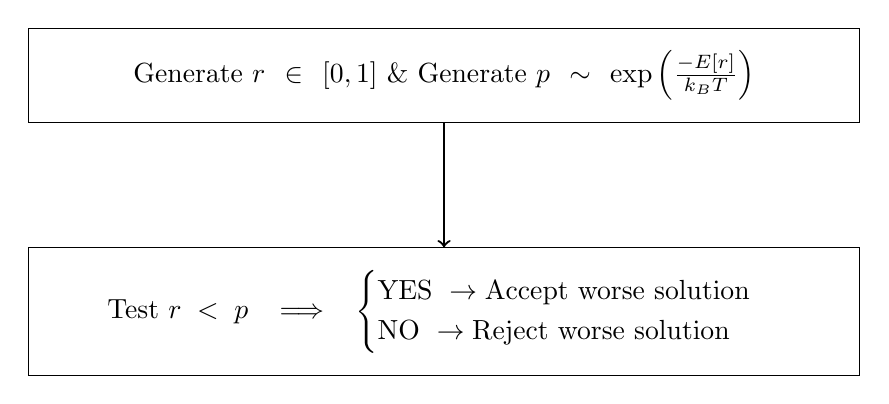
\begin{tikzpicture}[node distance=2.5cm, auto]
		% First box
	    \node[draw, text width=10cm, align=center, inner sep=8pt] (box_one) {
				Generate  \(r \in [0,1]\) \& Generate \(p \sim \exp \left( \frac{-E[r]}{k_B T} \right)\)
			};

		% Second box
		\node[draw, text width=10cm, align=center, inner sep=8pt, below of=box_one, yshift=-0.5cm] (box_two) {
					Test \( r < p \implies
					\begin{cases}
						\text{YES } \rightarrow \text{Accept worse solution} \\
						\text{NO } \rightarrow \text{Reject worse solution}
					\end{cases}
				\)
			};

	    % Arrow between boxes
		\draw[->, thick] (box_one) -- (box_two);
	\end{tikzpicture}
\end{figure}

Here:
\begin{itemize}
	\item \(E[r_i]\) is the energy of the configuration of cities, i.e. the distance of the current tour.
	\item \(k_B\) is the Boltzmann constant.
	\item \(T\) is the current temperature of the system.
\end{itemize}

From rudimentary statistics, the acceptance criterion is less enforced when the system is of low energy, and more possible to occur when there are higher temperatures in play. Lastly, this iterative process continues until a stopping criterion is reached, or a certain tolerance on the length of the final tour is achieved.

\subsection{Ant Colony Optimization}
\label{subsec: ACO}

Lastly, a famous heuristic family of algorithms comes from the Ant Colony systems of AC for short.

Ants in the real-world are capable of finding the shortest path from a food source back to their nest, without the uses of visual cues \cite{beckers1992trails}. This is achieved by depositing pheromone information as they walk, which eventually reinforces certain routes, and leads them to the optimal path back home.

Similarly, in the AC family of algorithms for the TSP, artificial ants cooperate to find the optimal solution of the problem, by exchanging information via pheromones deposited on graph edges (roads) \cite{dorigo1997ant}. This scheme, which has similarities with reinforcement learning procedures, takes into consideration the balance between heuristic information (shorter distances between two cities) and pheromone numbers deposited on edges by past iterations.

As such, each agent takes advantage of the deposited information by other ants on the graph, while also retaining the freedom to search an optimal path on its own. Thus, there is a balance here between exploration of new paths, and exploitation of previous knowledge. 

The algorithm works as follows. First, each ant generates a tour by choosing which city to visit next, by a \textbf{probabilistic city transition rule}. This rule favours ants which prefer to move to cities which are connected by short distances, with a high amount of pheromone.

Once all ants have completed their tour, a \textbf{global pheromone update rule} is applied. During this phase, a fraction of the deposited pheromone evaporates from all edges. This causes paths which are not preferred by many ants to become less desirable. In addition, each ant then deposits a small amount of pheromone on the edges that belong to its tour, in proportion to how \textit{short} the tour war. 

When the process if finished, the resulting edges that belong in small tours, receive the greatest amount of pheromones, reinforcing optimal choices for the next generation of ants to traverse the graph. This scheme is then re-iterated until a stopping criterion is met.
			% what heuristics will be used
% Limitation section of Final Essay for Math & Environment %
% Author: Konstantinos Garas
% E-mail: kgaras041@gmail.com // k.gkaras@student.rug.nl
% Created: Fri 28 Mar 2025 @ 15:52:26 +0100
% Modified: Sat 29 Mar 2025 @ 13:30:37 +0100

\section{Limitations}
\label{sec: limitations}

Apart from being only approximation algorithms, the families of  the numerical schemes that were introduced in the previous section have many limitations, most of which are prevalent in all individual implementation cases.

\subsection{Nearest Neighbour}
\textbf{Greedy, inaccurate but fast.}

Due to the symmetric nature of the case study, the NN algorithm was able to produce good results even for its greedy nature. In the literature however, there are many mathematicians who advise against the use of this algorithm, due to the sheer number of bad cases that exist, that make it achieve the worst possible results \cite{gutin2002traveling}.

\subsection{Genetic Algorithm}
\textbf{Initialization matters, performance considerations.}

Since it is up to the user to define an initial instance of the population, and efficient reproduction (also called crossover) and mutation operators, this algorithms can have significantly worse performance than all other candidates of this study. Its enormous uptime and worse results are evident in Section \ref{sec: results}. Lastly, to showcase how important is proper initialization for this algorithm, the Greedy Permuting Method \cite{liu2018greedy} is also tested, which produces much more acceptable results than the default GA.

\subsection{Simulating Annealing}
\textbf{Initialization matters, acceptance criterion as well.}

As Simulated Annealing is also an iterative algorithm, the initial solution that forms the basis of the algorithm has significant implications on its actual performance. In addition, the acceptance criterion is also something that requires careful consideration, especially when the algorithm accepts a worse solution than the one before. Simply put, we try to avoid having good solutions being overwritten by worse ones. Lastly, the algorithm produces better results as we increase the number of allowed iterations (the starting temperature).

\subsection{Ant Colony Optimization}
\textbf{Heavy on user defined parameters.}

The Ant Colony family has the problem of being very dependent on the choices made by the user. The decay rate of pheromones, the importance of heuristic information (distance) versus pheromone number, and even the city transition rule, are all values that depend on how the user implements them. It is evident that a more careful consideration of these parameters produces substantially better results.

In addition, the ACO family is also really diverse. Different arguments can be made for a global, versus a local, pheromone update rule. Moreover, it can also be modified with local search algorithms like \textbf{3-Opt}. This discussion is made by the original authors to great extent \cite{dorigo1997ant}.
			% limitations of each algorithm
% Results of the Final Essay for Math & Environment %
% Author: Konstantinos Garas
% E-mail: kgaras041@gmail.com // k.gkaras@student.rug.nl
% Created: Fri 28 Mar 2025 @ 16:05:36 +0100
% Modified: Sat 29 Mar 2025 @ 13:48:13 +0100

\section{Comparison of the Algorithms}
\label{sec: results}
The heuristic algorithms that were described in Section \ref{sec: heuristics} are now compared in terms of their performance for 30 randomly generated graphs of 229 cities, a size of which is equivalent to the size of the Netherlands. 

Table \ref{table: nicknames} provided a legend for the nicknames of the algorithms in the figures, while figures \ref{fig: mean_distance}, \ref{fig: mean_uptime}, \ref{fig: min_distance} compare the algorithms in terms of \textit{mean distance, mean uptime, minimum distance achieved} respectively. Lastly, figure \ref{fig: compare_all} groups all the results together for a more cohesive view.

\subsection{Technical Information}
The algorithms were implemented in \texttt{Python 3.12.3} with the only materials to be used being the pseudo-codes in the original papers. Then, the case study was run in the Hábrók High Performance Computing cluster of the University of Groningen, over the period of 16 hours, with 5 processing cores working at 100\%. Due to the intense nature of the computations, I strongly recommend not to run these programs in a normal computer.

\begin{table}[htbp]
	\centering
	\begin{tabular}{|c|c|}
		\hline
		\textbf{Algorithm}	&	\textbf{Figure Name} \\
		\hline
		Nearest Neighbour  & NN \\
		Baseline Genetic Algorithm	&	BGA	\\
		Genetic Algorithm	&	GA	\\
		Greedy Permuting Method	&	GPM	\\
		Baseline Simulated Annealing	&	BSA	\\
		Simulated Annealing	&	SA	\\
		Baseline Ant Colony Optimization	&	BACO	\\
		Ant Colony Optimization	&	ACO \\
		\hline
	\end{tabular}
	\caption{Table of names used in the following figures.}
	\label{table: nicknames}
\end{table}

\begin{itemize}
	\item \textbf{Baseline GA, SA, ACO:} The results are generated without fine-tuning of the user-defined parameters\footnote{The Nearest Neighbour algorithm doesn't accept user defined parameters, and as such, it can't be fine-tuned}.
	\item \textbf{GA, SA, ACO:} These algorithms have been fine-tuned in terms of the optimal output. Speed was entirely sacrificed in order to get the best possible final tour in each test.
\end{itemize}

\begin{figure}[htbp]
	\centering
	\includegraphics[width=0.7\textwidth]{Extras/Comparison_Mean_Distance.png}
	\caption{Comparison of the heuristic algorithms in terms of Mean Distance, after 30 randomly generated experiments. Fine-tuned Ant Colony Optimization produced the best results.}
	\label{fig: mean_distance}
\end{figure}

\begin{figure}[htbp]
	\centering
	\includegraphics[width=0.7\textwidth]{Extras/Comparison_Mean_Uptime.png}
	\caption{Comparison of the Mean Uptime of the heuristic algorithms, after 30 randomly generated experiments. Here, NN is the fastest of all other choices by a large margin.}
	\label{fig: mean_uptime}
\end{figure}

\begin{figure}[htbp]
	\centering
	\includegraphics[width=0.7\textwidth]{Extras/Comparison_Min_Distance.png}
	\caption{Comparison of the Minimum Distance achieved by the heuristic algorithms, after 30 randomly generated experiments. Once more, Ant Colony Optimization produced the best possible answer.}
	\label{fig: min_distance}
\end{figure}

\begin{figure}[h]
	\centering
	\includegraphics[width=0.7\textwidth]{Extras/Comparison_All.png}
	\caption{A final figure showcasing the Mean Distance, and Mean Uptime achieved for each heuristic algorithm in the case study.}
	\label{fig: compare_all}
\end{figure}
				% numerical results
% Conclusion of the Final Essay for Math & Environment %
% Author: Konstantinos Garas
% E-mail: kgaras041@gmail.com // k.gkaras@student.rug.nl
% Created: Fri 28 Mar 2025 @ 16:23:50 +0100
% Modified: Sat 29 Mar 2025 @ 13:48:21 +0100

\section{Conclusion}
\label{sec: conclusion}

To conclude, this case study has introduced the famous algorithmic families that are used to solve the Travelling Salesman Problem. Each heuristic family is comparable and stems from various different concepts already in place in nature. Unfortunately for us, this doesn't mean that the great ideas described in this report can have any effect at solving other similarly hard problem of the scientific world.

As a final remark, I would like to close the case study by my personal opinion on the subject. Overall, as a scientist, I like both the Simulated Annealing and the Ant Colony algorithms. The first, because I find it very easy to combine it with other well established algorithms in the field of discrete optimization \cite{ye2013improved}, while the latter because of its ingenious observation of how ants search for food.

Additionally, a more efficient manual implementation of these algorithms, for example in \texttt{C} or \texttt{Rust}, or by someone with a more refined coding experience, would produce results much more compatible with standard academic practices. Unfortunately, the timetables of such a project is out of the scope of 1 week, which was the time used to develop the source files.
			% conclusion with opinion

% Manage references and plug them into the table of contents.
\addcontentsline{toc}{section}{References}
\bibliographystyle{unsrt}
\bibliography{/home/anenin/Documents/Projects/LaTeX/templates/article/references.bib}

\end{document}
